\chapter{METODOLOGIA}

As seções a seguir apresentarão a metodologia adotada neste trabalho. Nelas serão 
trabalhados temas como o tipo da pesquisa (\autoref{sec:objetivos}), as etapas definidas para a construção do 
presente estudo (seção ), bem como os materiais necessários para o desenvolvimento do protótipo 
(seção 3.3).

\section{Tipo de pesquisa}

\lipsum[2]

\section{Etapas da pesquisa}

\lipsum[1]

\subsection{Etapa 1 – Levantamento bibliográfico}

\lipsum[2]

\subsection{Etapa 2 – Seleção de ferramentas e dispositivos}

\lipsum[1]

\begin{itemize}
  \item Sensor de efeito Hall (para medir a rotação da roda e estimar a distância percorrida);
  \item Módulo MPU-6050 (para medir aceleração e variação angular);
  \item Microcontrolador ESP32 (para processamento e envio dos dados);
  \item Power bank (para alimentação do sistema).
\end{itemize}

\begin{figure}[H]
  \centering
  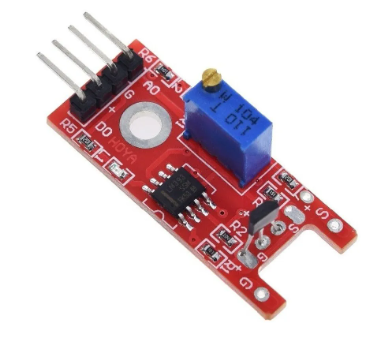
\includegraphics[width=0.7\textwidth]{figuras/sensorhall.png}
  \caption{Sensor de efeito Hall utilizado para medição de rotação.}
  \label{fig:sensor-hall}
  \fonte{Imagem elaborada por Tauan Anjos (2026).}
\end{figure}


\begin{figure}[H]
  \centering
  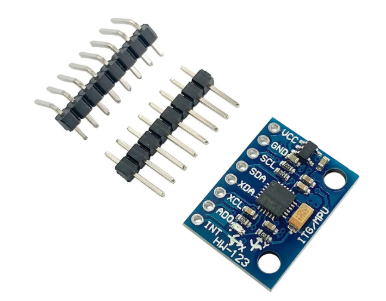
\includegraphics[width=0.7\textwidth]{figuras/mpu.png}
  \caption{Módulo inercial MPU-6050 para medição de aceleração e variação angular.}
  \label{fig:sensor-mpu}
  \fonte{Imagem elaborada por Tauan Anjos (2026).}
\end{figure}


\begin{figure}[H]
  \centering
  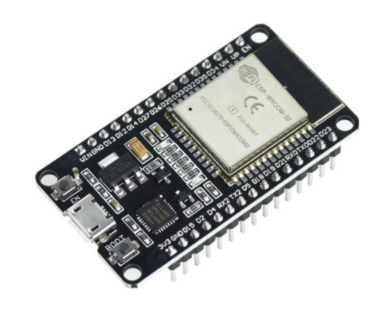
\includegraphics[width=0.7\textwidth]{figuras/esp32.png}
  \caption{Microcontrolador ESP32 utilizado para processamento de dados.}
  \label{fig:esp32}
  \fonte{Imagem elaborada por Tauan Anjos (2026).}
\end{figure}

\lipsum[1]

\subsection{Etapa 3 – Desenvolvimento e integração do protótipo}

\lipsum[1]

\subsection{Etapa 4 – Testes conceituais}

\lipsum[1]

\subsection{Etapa 5 – Análise e interpretação dos dados}

\lipsum[1]
 
\section{Ferramentas e materiais necessários}

\lipsum[1]

\begin{itemize}
  \item Hardware: Sensor Hall, MPU-6050, microcontrolador ESP32, power bank, cadeira de rodas manual, suporte para fixação dos sensores.
  \item Software: Arduino IDE, planilhas eletrônicas (Excel ou Google Sheets), eventualmente softwares complementares para análise dos dados.
\end{itemize}


\chapter{DESENVOLVIMENTO}\label{cap:desenvolvimento}

\lipsum[1]

\section{Levantamento bibliográfico}

\lipsum[1]

\section{Seleção de ferramentas e sensores}
\lipsum[5]

\section{Arquitetura do protótipo e cálculos implementados}

\lipsum[3]

\begin{equation}
V = P
\end{equation}
em que \(P\) representa o número total de pulsos detectados.

A distância percorrida \(D\) é obtida a partir da multiplicação do número de voltas pela circunferência da roda \(C\):
\begin{equation}
D = V \times C
\end{equation}

A velocidade linear é calculada com base no tempo entre dois pulsos consecutivos \(\Delta t\), correspondente ao tempo necessário para uma rotação completa da roda. A velocidade em rotações por segundo é dada por:
\begin{equation}
RPS = \frac{1}{\Delta t}
\end{equation}

A velocidade linear em metros por segundo é calculada por:
\begin{equation}
v = RPS \times C
\end{equation}

Para conversão da velocidade para quilômetros por hora, utiliza-se:
\begin{equation}
v_{km/h} = v \times 3{,}6
\end{equation}

\lipsum[3]


\begin{table}[h!]
\centering
\caption{Esquema de ligação elétrica dos sensores ao ESP32}
\label{tab:ligacao_sensores}
\begin{tabular}{|l|c|c|l|}
\hline
\textbf{Dispositivo} & \textbf{Pino do Módulo} & \textbf{Pino do ESP32} & \textbf{Função} \\ \hline
MPU6050 & VCC & 3V3 & Alimentação 3.3V \\ \hline
MPU6050 & GND & GND & Referência comum \\ \hline
MPU6050 & SDA & GPIO 21 & Dados I2C \\ \hline
MPU6050 & SCL & GPIO 22 & Clock I2C \\ \hline
Sensor Hall & VCC & 3V3 & Alimentação 3.3V \\ \hline
Sensor Hall & GND & GND & Referência comum \\ \hline
Sensor Hall & OUT & GPIO 27 & Pulso digital \\ \hline
\end{tabular}
\end{table}


\lipsum[1]

\section{Implementação do circuito e testes experimentais}

A implementação do protótipo iniciou-se com a montagem do circuito  em conjunto com o microcontrolador ESP32, conforme ilustrado na \autoref{fig:hall-esp32}. \lipsum[1]

\lipsum[7]

\begin{figure}[H]
  \centering
  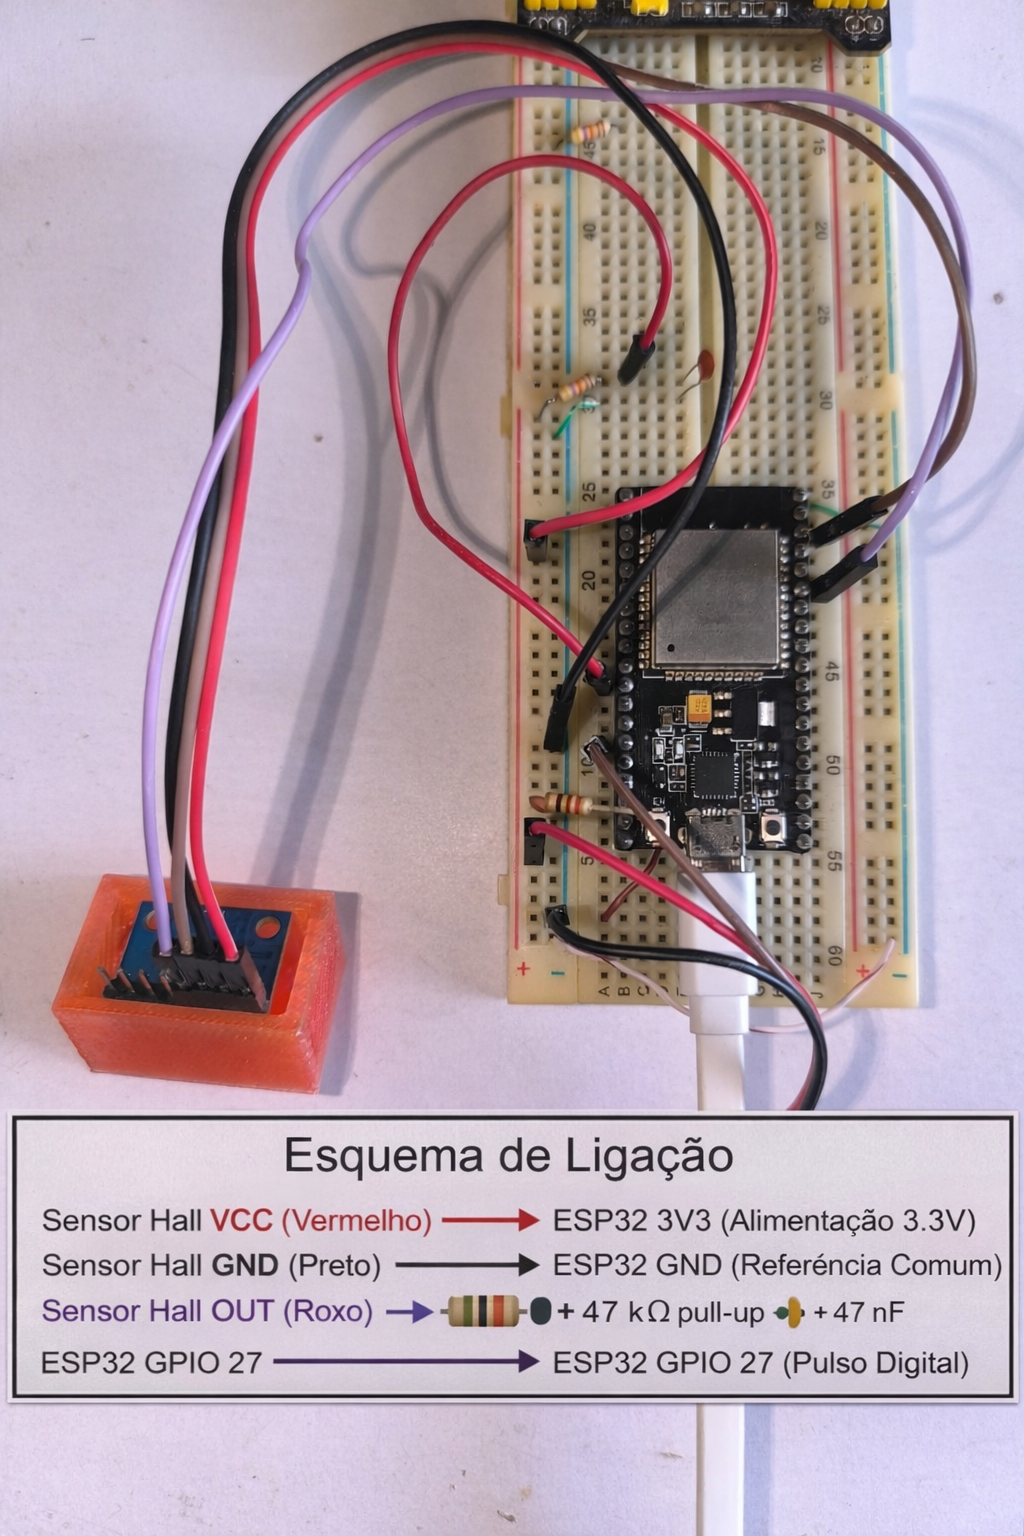
\includegraphics[width=0.7\textwidth]{figuras/esquema-eletrico.png}
  \caption{Montagem do circuito com sensor de efeito Hall, resistor de pull-up e capacitores de filtragem conectados ao ESP32.}
  \label{fig:hall-esp32}
  \fonte{Gustavo Passos (2026), com edição do autor.}
\end{figure}

\section{Implementação física e adaptação à cadeira de rodas}

\lipsum[2]

\begin{figure}[H]
  \centering
  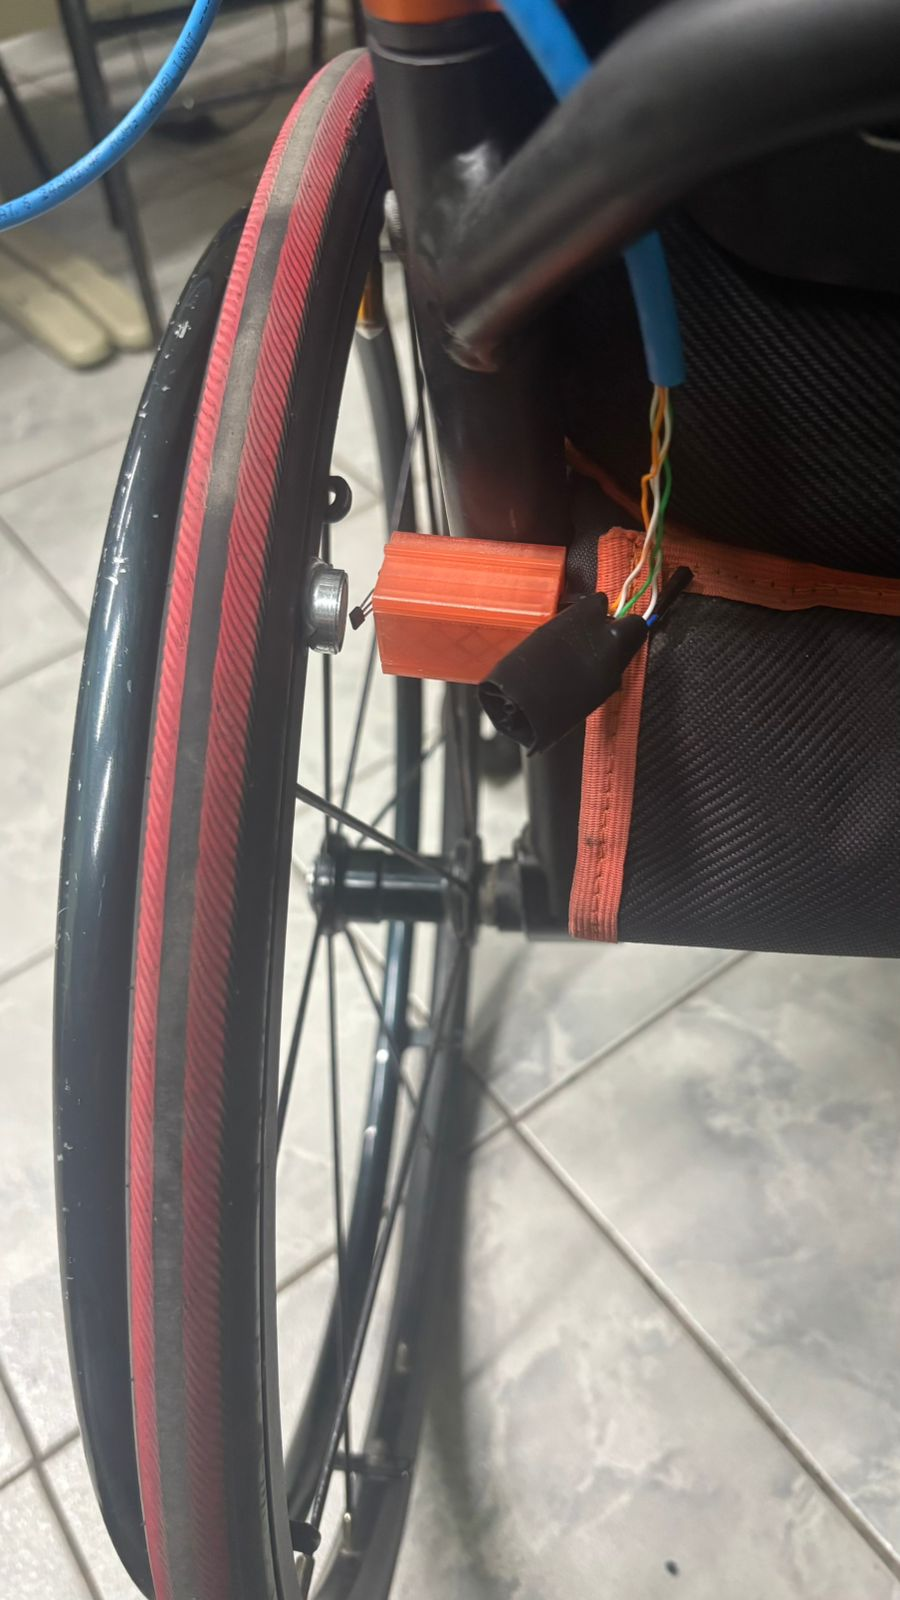
\includegraphics[width=0.5\textwidth]{figuras/sensor-hall-cadeira.jpg}
  \caption{Fixação do sensor de efeito Hall na estrutura da cadeira de rodas e posicionamento do ímã na roda.}
  \label{fig:hall-cadeira}
  \fonte{Imagem elaborada pelo autor (2026).}
\end{figure}


\lipsum[1]

\begin{figure}[H]
  \centering
  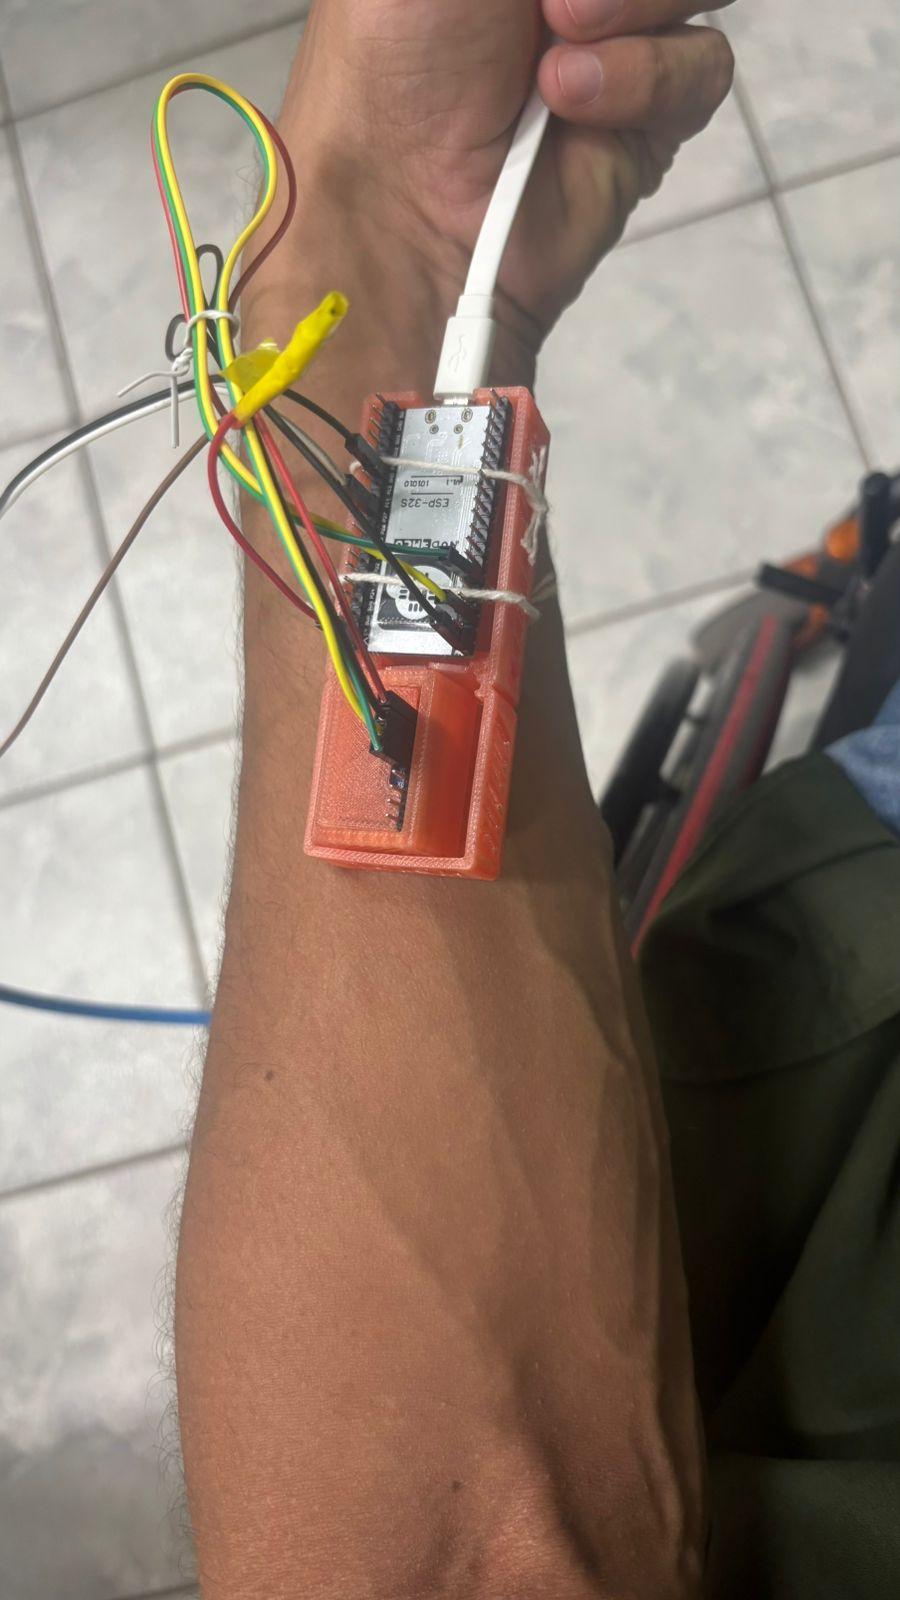
\includegraphics[width=0.5\textwidth]{figuras/esp32-mpu-braco.jpg}
  \caption{Protótipo contendo o ESP32 e o módulo MPU-6050 fixados ao antebraço do usuário.}
  \label{fig:esp32-braco}
  \fonte{Imagem elaborada pelo autor (2026).}
\end{figure}


\lipsum[1]

\section{Interface de visualização e telemetria dos dados}

\lipsum[4]

As \autoref{fig:dashboard-movimento} e~\autoref{fig:dashboard-parado} apresentam o painel em operação nos estados de movimento e repouso, respectivamente.

\begin{figure}[H]
  \centering
  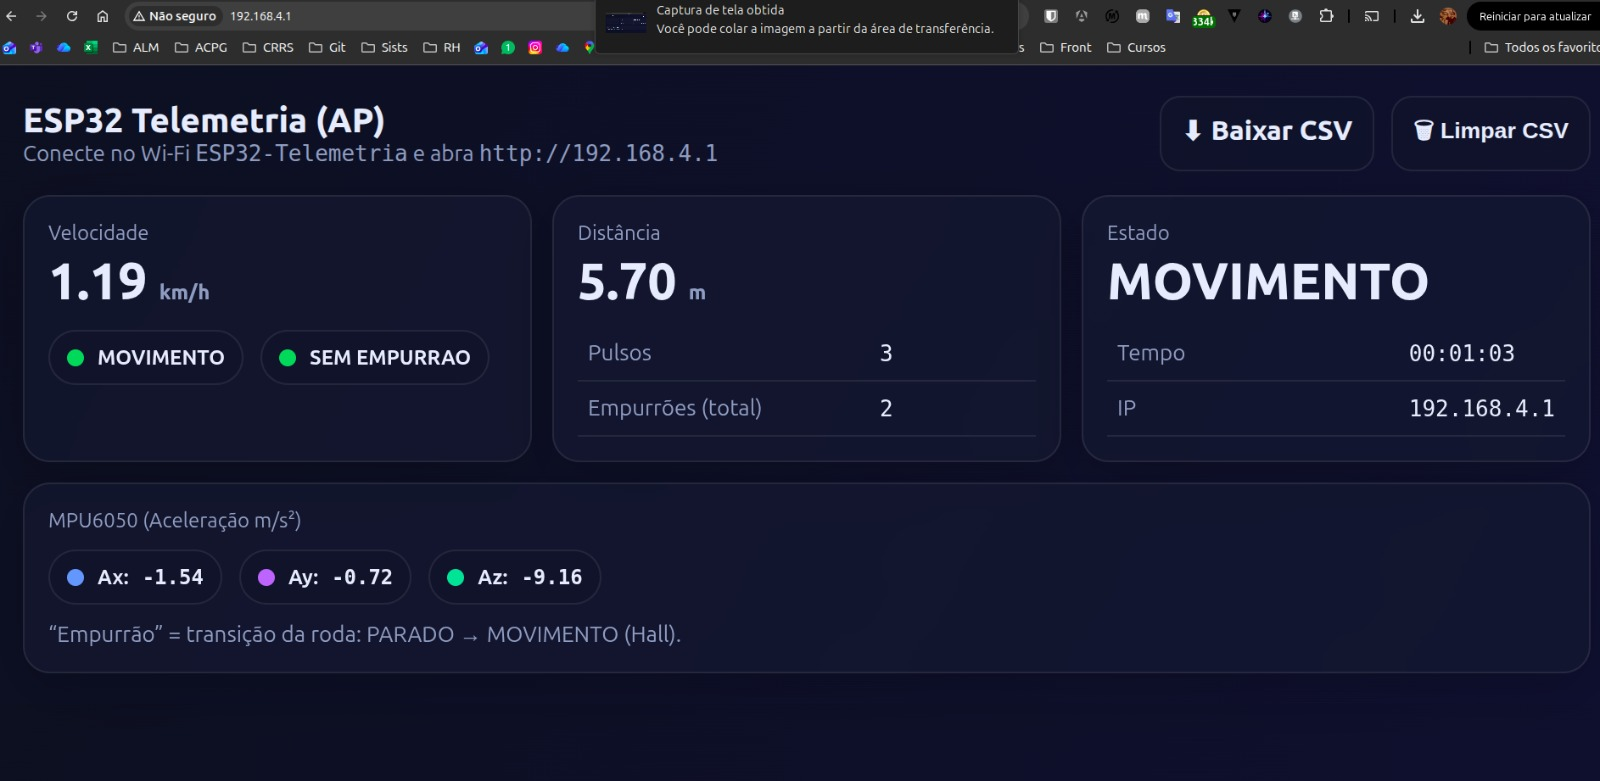
\includegraphics[width=0.6\textwidth]{figuras/dashboard-tcc-movimento.jpg}
  \caption{Dashboard em operação durante o estado de movimento, exibindo velocidade, distância e dados do MPU-6050.}
  \label{fig:dashboard-movimento}
  \fonte{Imagem elaborada pelo autor (2026).}
\end{figure}

\begin{figure}[H]
  \centering
  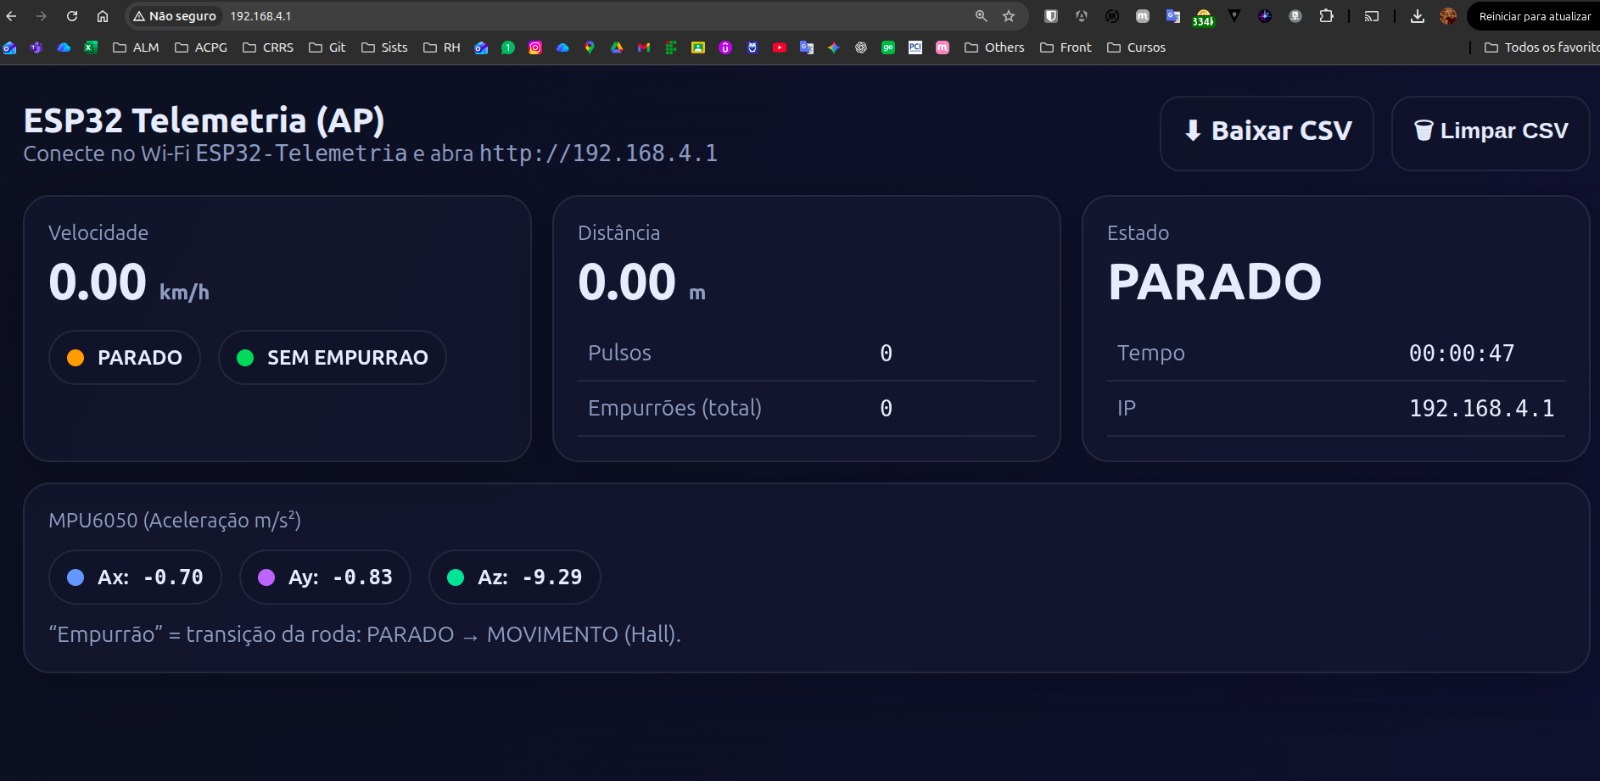
\includegraphics[width=0.6\textwidth]{figuras/dashboard-tcc.jpg}
  \caption{Dashboard no estado de repouso, indicando velocidade nula e ausência de pulsos detectados.}
  \label{fig:dashboard-parado}
  \fonte{Imagem elaborada pelo autor (2026).}
\end{figure}


